% ex: ts=2 sw=2 sts=2 et filetype=tex
% SPDX-License-Identifier: CC-BY-SA-4.0
\begin{frame}
    \frametitle{Contenido}
    \tableofcontents
\end{frame}

\section{Análisis del problema}

\begin{frame}[c]{¿Qué haremos en este curso?}
  A partir de la descripción y análisis de un problema
  \pausa
  \begin{enumerate}
    \item Diseñar la solución mediante
      \begin{itemize}
        \item Pseudocódigo
        \item Diagrama de flujo
      \end{itemize}
    \pausa
    \item Codificar la solución utilizando
      \begin{itemize}
        \item Lenguaje de programación \textbf{Python}
      \end{itemize}
    \pausa
    \item Probar que funciona con un conjunto de datos de prueba
  \end{enumerate}
\end{frame}

\begin{frame}[c]{¿Qué haremos en este curso?}
  A partir de un algoritmo (pseudocódigo o diagrama de flujo)
  \begin{enumerate}
    \item Explicar qué hace el algoritmo
    \pausa
    \item Cuáles son las salidas esperadas a partir de ciertos datos de
      entrada
    \pausa
    \item ¿Qué se tiene que cambiar para atender un nuevo requerimiento?
  \end{enumerate}
\end{frame}

\begin{frame}[c]{Tipos de problema a resolver}
  \pausa
  \begin{itemize}
    \item Aquellos que pueden resolverse mediante una o más operaciones:
      \begin{enumerate}
        \item Aritméticos (suma, resta, multiplicación, división, residuo,
          a nivel de bits)
        \pausa
        \item Relacionales y lógicos (mayor, menor, diferente, igual, Y, O, NO)
        \pausa
        \item De asignación (un valor se guarda en una variable)
        \pausa
        \item Entrada de datos (se leen los datos del teclado, archivos, BD,
          algún dispositivo)
        \pausa
        \item Salida de datos (se escriben los datos en la pantalla, archivos,
          BD, dispositivo)
      \end{enumerate}
    \pausa
    \item Aquellos que se pueden ejecutar de manera secuencial
    \pausa
    \item Aquellos que se pueden ejecutar sólo si se cumple alguna condición
    \pausa
    \item Aquellos que se pueden ejecutar tantas veces mientras se cumpla una
      condición
    \pausa
    \item Aquellos que se puedan organizar en módulos
  \end{itemize}
\end{frame}

\begin{frame}[c]{Fases del desarrollo de programas}
  \begin{description}
    \item[Descripción del problema] Especificaciones de lo que se pretende
      resolver.
    \pausa
    \item[Análisis del problema] Descripción de la funcionalidad del programa.
      Características, entradas y salidas, cálculos, tipos de datos,
      restricciones, etc.
    \pausa
    \item[Diseño del algoritmo] Modelado de la solución. Representación
      textual (pseudocódigo) o gráfica (Diagramas de flujo) de la solución.
    \pausa
    \item[Programación y pruebas] Codificación del algoritmo diseñado en un
      lenguaje de programación. Prueba y depuración de errores.
    \pausa
    \item[Mantenimiento del programa] Adaptación del programa a las nuevas
      necesidades.
  \end{description}
\end{frame}

\section{Pseudocódigo y diagramas de flujo}

\begin{frame}[fragile]
  \frametitle{Pseudocódigo}
  \begin{itemize}
    \item Descripción textual del algoritmo independientemente de cualquier
      lenguaje de programación
    \pausa
    \item Es una descripción detallada de alto nivel, legible, compacta e
      informal
    \pausa
    \item Descripción expresada en lenguaje natural y no en un lenguaje de
      programación
    \pausa
    \item Omite declaración de variables y código específico del sistema
  \end{itemize}
  \pausa
  Ejemplo:
  \begin{lstlisting}[style=pseudocodigo]
Algoritmo suma_de_dos_numeros
  Escribir "Dame el primer número"
  Leer N1
  Escribir "Dame el segundo número"
  Leer N2
  Suma <- N1 + N2
  Escribir "El resutlado es:", Suma
FinAlgoritmo
  \end{lstlisting}
\end{frame}

\begin{frame}[c]{Diagrama de flujo}
  \begin{columns}
    \column{0.5\textwidth}
      \begin{center}
        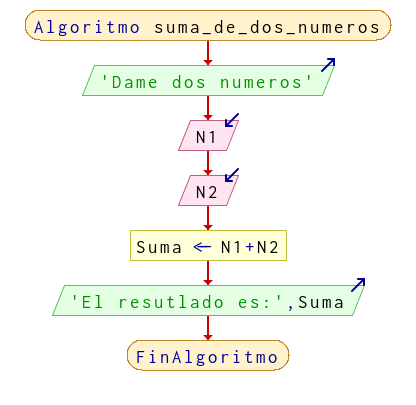
\includegraphics[scale=0.5]{012-df_suma.png}
      \end{center}
    \column{0.5\textwidth}
      \begin{itemize}
        \item Es la representación gráfica de un algoritmo
        \pausa
        \item Algoritmo descrito mediante formas geométricas y flechas que las unen
        \pausa
        \item Es una alternativa al uso del pseudocódigo que representa con mayor
          claridad la secuencia de instrucciones y los caminos posibles que puede
          seguir un algoritmo
        \pausa
        \item Es muy útil cuando el algoritmo incluye decisiones o repeticiones
      \end{itemize}
  \end{columns}
\end{frame}

\begin{frame}[c]{Diagrama de flujo}
  \begin{columns}
    \column{0.5\textwidth}
      \begin{center}
        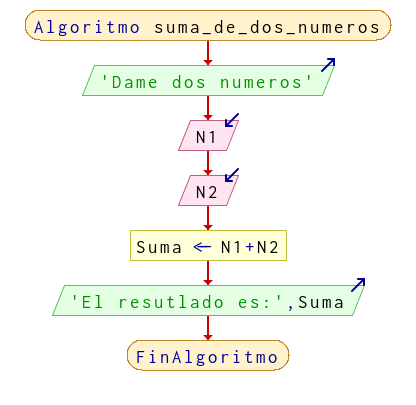
\includegraphics[scale=0.5]{012-df_suma.png}
      \end{center}
    \column{0.5\textwidth}
      \begin{itemize}
        \item Propone un símbolo particular para cada tipo de operación efectuada
        \pausa
        \item Cada símbolo incluye el texto que expresa la operación realizada
        \pausa
        \item Los símbolos se unen mediante flechas que indican el sentido, es
          decir, qué cosa se hace primero y qué se hace después
        \pausa
        \item Si ya no hay espacio, se pueden utilizar conectores
      \end{itemize}
  \end{columns}
\end{frame}

%\begin{frame}[c]{Simbología}
%\end{frame}

\begin{frame}[c]{Reglas de los diagramas de flujo}
  \begin{columns}
    \column{0.5\textwidth}
      \begin{center}
        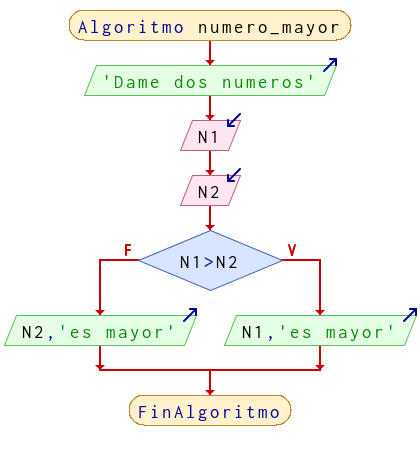
\includegraphics[scale=0.4]{012-df_num_mayor.png}
      \end{center}
    \column{0.5\textwidth}
      Algunas reglas de construcción:
      \begin{itemize}
        \item Un solo símbolo de inicio y un solo símbolo de fin
        \pausa
        \item Todos los símbolos deben estar conectados con flechas
        \pausa
        \item Todos los flujos entran por arriba del símbolo y salen por debajo
          o un costado
        \pausa
        \item Los flujos no se inclinan ni cruzan, y se realizan en ángulos de 90°
      \end{itemize}
  \end{columns}
\end{frame}

\begin{frame}[c]{Reglas de los diagramas de flujo}
  \begin{columns}
    \column{0.5\textwidth}
      \begin{center}
        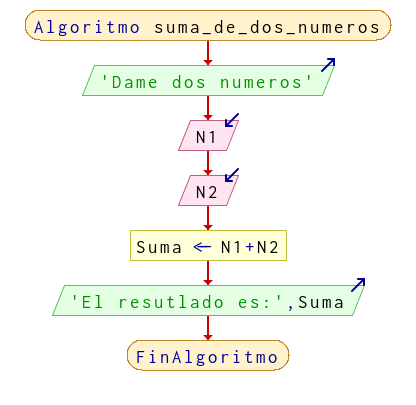
\includegraphics[scale=0.5]{012-df_suma.png}
      \end{center}
    \column{0.5\textwidth}
      Algunas reglas de construcción:
      \begin{itemize}
        \item A cada símbolo sólo entra un flujo
        \pausa
        \item El diagrama se desarrolla de arriba abajo y de izquierda a derecha
        \pausa
        \item Usar el mínimo de palabras dentro de los símbolos y notación matemática
      \end{itemize}
  \end{columns}
\end{frame}

%\section{Herramientas computacionales para ejecutar pseudocódigos y
%diagramas de flujo}

%\begin{frame}[c]{Conceptos}
  %\begin{itemize}
    %\item a
  %\end{itemize}
%\end{frame}

\begin{frame}[c]{Ejercicio}
  Escribir un algoritmo para los siguientes puntos, y representar también en
  diagrama de flujo.
  \begin{enumerate}
    \item Determinar el número mayor de dos números enteros.
    \item Determinar si un número es par o no.
    \item Calcular el descuento de un producto. Aplicar un 50\% + 20\% al
      precio de lista del producto.
  \end{enumerate}
\end{frame}
